%$Id: interp.tex,v 1.1 1992/05/10 19:42:22 rz Exp rz $
\chapter{Univariate Interpolation}
\label{Interpolation:Chap}

The previous chapter showed how to determine if a polynomial was zero
by examining its values at well chosen points.  This chapter develops
techniques to determine the polynomial itself from a sequence of 
values.  This process is called {\em interpolating a polynomial
from its values\/}.  This technique is one of the most useful tools
for constructing efficient symbolic computing algorithms for sparse problems.

In the previous chapter we used knowledge about when Vandermonde matrices
were non-singular to develop deterministic algorithms for zero
testing.  In this chapter we will also need to solve systems of
linear equations whose coefficients form a Vandermonde matrix.
\sectref{Vandermonde:Sec} develops some properties of Vandermonde
matrices and the basic techniques for dealing with Vandermonde style
systems of equations.

We consider two interpolation schemes for univariate polynomials in
the chapter, the \keyi{Lagrange interpolation formula} and the
\keyi{Newton interpolation formula}.  The Lagrange technique follows
directly from Vandermonde techniques discussed in
\sectref{Vandermonde:Sec} and are discussed in
\sectref{Interp:Lagrange:Sec}.  The Newton interpolation scheme arises 
from applying the Chinese remainder algorithm\index{Chinese remainder
theorem} to the values of a polynomial.  It is discussed in
\sectref{Interp:CRA:Sec}.

By choosing the evaluation points in an interpolation scheme
especially carefully, it is possible to interpolate exceedingly
quickly.  This technique, the \key{fast Fourier transform}, is
discussed in \sectref{Poly:FFT:Sec} and is applied to multiplying
polynomials.  This produces the fastest known polynomial multiplication
algorithm.  The complexities of these different algorithms is
summarized in \figref{Interp:Complex:Fig}.

\begin{figure}
\begin{center}
\begin{tabular}{|c|c|c|}
\multicolumn{1}{c}{Algorithm} & \multicolumn{1}{c}{Time} 
  & \multicolumn{1}{c}{Space} \\ \hline
Lagrange & $O(n^2)$ & $O(n)$ \\ \hline
Newton & $O(n^2)$ & $O(n)$ \\ \hline
Fast Fourier  & $O(n \log n)$ & $O(n)$ \\ \hline
\end{tabular}
\end{center}
\caption{Complexity of different interpolation
algorithms\label{Interp:Complex:Fig}}
\end{figure}


In \sectref{Interp:Abstract:Sec} we discuss interpolation from a
somewhat more abstract perspective.  This approach allows us to
combine the Chinese remainder theorem results for integers with those
for polynomials into a single uniform framework.

\section{Vandermonde Matrices}
\label{Vandermonde:Sec}

\index{Vandermonde matrix|(}

Vandermonde matrices have two properties that make them particularly
useful for the algorithms in this chapter: (1) it is easy to ensure
that they are non-singular and (2) systems of linear equations whose
coefficients form Vandermonde matrices are easy to solve exactly. Note
that Vandermonde matrices of floating point numbers can be numerically
quite unstable and these techniques may not be appropriate.

A \keyi{Vandermonde matrix} is a matrix of the form  
\begin{equation} \label{Vandermonde:Eq}
V_n = \begin{pmatrix}
1& k_1 & k_1^2 & \cdots & k_1^{n-1}\\
1& k_2 & k_2^2 & \cdots & k_2^{n-1}\\
\vdots& &\vdots& & \vdots\\
1& k_n & k_n^2 & \cdots & k_n^{n-1}\end{pmatrix},
\end{equation}
where the $k_i$ are chosen from some field.
Similarly, a system of linear equations of the form
\[
\begin{aligned}
X_1 + k_1 X_2 + k_1^2 X_3 + \cdots + k_1^{n-1} X_n &= w_1 \\
X_1 + k_2 X_2 + k_2^2 X_3 + \cdots + k_2^{n-1} X_n &= w_2 \\
\vdots&\\
X_1 + k_n X_2 + k_n^2 X_3 + \cdots + k_n^{n-1} X_n &= w_n 
\end{aligned}
\]
will be called a \keyi{Vandermonde system of equations}.

A matrix where the degrees of each column are the same and within each
row the degrees rise monotonically, is called a {\em generalized
Vandermonde matrix\/},\index{Vandermonde matrix!generalized} \viz,
\[
\begin{pmatrix}
k_1^{e_1}& k_1^{e_2} & k_1^{e_3} & \cdots & k_1^{e_n}\\
k_2^{e_1}& k_2^{e_2} & k_2^{e_3} & \cdots & k_2^{e_n}\\
\vdots& &\vdots& & \vdots\\
k_n^{e_1}& k_n^{e_2} & k_n^{e_3} & \cdots & k_n^{e_n}\end{pmatrix},
\]
where $e_1 < e_2 < \cdots e_n$.  We will often use generalized
Vandermonde matrices where $e_1 = 0$.

The determinant of a \key{Vandermonde matrix} is particularly simple
to compute.  Multiplying the $i$-th column of
\eqnref{Vandermonde:Eq} by $k_1$ and subtracting it from the
$i+1${\st} column gives,
\[
\det V_n = 
  \left|
  \begin{array}{ccccc}
    1&0&0 &\cdots &0\\
    1&k_2 - k_1&k_2^2 -k_1 k_2& \cdots &k_2^{n-1} - k_2^{n-2} k_1 \\
    \vdots&\vdots&\vdots&  & \vdots\\
    1&k_n - k_1&k_n^2 -k_1 k_n& \cdots &k_n^{n-1} - k_n^{n-2} k_1 
  \end{array}\right|.
\]
Expanding by \keyi{Cramer's rule} across the first row and factoring out
$k_i-k_1$ from the $i$-th row we have the following recursive
formula
\[
\begin{aligned}
\det V_n &= \det V_{n-1} \prod_{1<j \le n} \left(k_j - k_1\right), \\
  & = \det V_{n-2} \prod_{2<j \le n} \left(k_j - k_2\right) 
      \prod_{1<j \le n} \left(k_j - k_1\right).
\end{aligned}   
\]
Thus we have:

\begin{proposition}
The determinant of the \key{Vandermonde matrix} is
\[
\det V_n = \prod_{1 \le i < j \le n} \left(k_j - k_i\right).
\]
\end{proposition}

\noindent
As an immediate consequence, the determinant of a \key{Vandermonde matrix}
is non-zero if and only if the $k_i$ are distinct.

\medskip
This result is not true for generalized Vandermonde matrices.  For
instance, for order $2$ matrices we have 
\[
\det V_{2} = 
\left|
\begin{array}{cc}
 1&k_1^e \\ 1 &k_2^e
\end{array}\right| = k_2^e - k_1^e,
\]
which implies that $V_{2}$ is nonsingular if and only if $k_{1}/k_{2}$
is not an $e$-th root of unity.  This is a stronger requirement
than was required for Vandermonde determinants.  In fact, an $n
\times n$ generalized Vandermonde determinant is divisible by the
related Vandermonde determinant.  

Nonetheless, a similar result on the singularity of generalized
Vandermonde matrices over the {\em reals\/}
is true, but the proof is a little trickier.  The following
proposition is only valid over $\R$, which has characteristic zero.
We know of no similar result for fields of positive characteristic.
        
\begin{proposition}
\label{Gen:Vandermonde:Prop}
The determinant of a generalized Vandermonde matrix is non-zero if the
$k_i$ are distinct positive real numbers.
\end{proposition}

\begin{proof}
We show the matrix is non-singular by induction.  A Vandermonde matrix
of order 1 is obviously non-singular since we only allow positive entries.
In the general case we consider a matrix of the form
\[
\begin{pmatrix}
1& k_1^{e_2} & k_1^{e_3} & \cdots & k_1^{e_n}\\
1& k_2^{e_2} & k_2^{e_3} & \cdots & k_2^{e_n}\\
\vdots& &\vdots & & \vdots\\
1& k_n^{e_2} & k_n^{e_3} & \cdots & k_n^{e_n}
\end{pmatrix}.
\]
Replace $k_1$ by the indeterminate $Z$ and consider the number of zeroes of
the polynomial
\[
G(Z) = 
\left|\begin{array}{ccccc}
  1& Z^{e_2} & Z^{e_3} & \cdots & Z^{e_n}\\
  1& k_2^{e_2} & k_2^{e_3} & \cdots & k_2^{e_n}\\
  \vdots& &\vdots & &\vdots\\
  1& k_n^{e_2} & k_n^{e_3} & \cdots & k_n^{e_n}
\end{array}\right| =
a_1 - a_2 Z^{e_2} + a_3 Z^{e_3} - \cdots - a_n Z^{e_n}.
\]
Each coefficient ($a_i$) is a minor of the original matrix and is itself a\Marginpar{This paragraph needs to be fixed up.}
generalized Vandermonde matrix of order $n-1$.  If $k_2, k_3, \ldots , k_n$
are distinct positive numbers then the minors are non-zero by induction.
The polynomial in $Z$ can only have $n-1$ positive zeroes by
\longpropref{Positive:Zeroes:Prop}.  But certainly each of $k_2, k_3, \ldots,
k_n$ is a zero of the polynomial.  Thus there are no other positive
real zeroes and $G(k_1) \not= 0$.
\end{proof}

The inverse of a \key{Vandermonde matrix} can be computed by the
following technique.  Multiply a Vandermonde matrix by a general $n$
by $n$ matrix:
\begin{equation}\label{Vander:InvProd:Eq}
\begin{pmatrix}
1&k_1&k_1^2&\cdots&k_1^{n-1}\\
1&k_2&k_2^2&\cdots&k_2^{n-1}\\
\vdots& & \vdots& & \vdots\\
1&k_n&k_n^2&\cdots&k_n^{n-1}
\end{pmatrix} \cdot
\begin{pmatrix}
p_{11}&p_{12}&p_{13}&\cdots&p_{1n}\\
p_{21}&p_{22}&p_{23}&\cdots&p_{2n}\\
\vdots& & \vdots& &\vdots\\
p_{n1}&p_{n2}&p_{n3}&\cdots&p_{nn}
\end{pmatrix},
\end{equation}
where the $p_{ij}$ are chosen such that this product is equal to the
identity matrix.
The $j$-th element of the top row of the product of these two matrices is
\[
p_{1j} + p_{2j} k_1 + p_{3j} k_1^2 + \cdots + p_{nj} k_1^{n-1} = P_j(k_1),
\]
where $P_j(Z)$ is a polynomial of degree $n-1$ in $Z$.
So, the product \eqnref{Vander:InvProd:Eq} is equal to 
\[
\begin{pmatrix}P_1(k_1)& P_2(k_1) & \cdots & P_n(k_1)\\
P_1(k_2)& P_2(k_2) & \cdots & P_n(k_2)\\
\vdots & \vdots & & \vdots\\
P_1(k_n)& P_2(k_n) & \cdots & P_n(k_n)\end{pmatrix}.
\]
By choosing $P_i(Z)$ such that $P_i(k_j) = 0$ if $i\not= j$ and
$P_i(k_i) =1$ otherwise, the above matrix becomes the identity matrix.
We let $P_j(Z)$ be
\begin{equation} \label{Vander:Pj:Eq}
P_j(Z) = \prod_{\genfrac{}{}{0pt}{2}{i \not= k}{1 \le i \le n}}
  {Z - k_i \over k_j - k_i}.
\end{equation}
The numerator ensures that the off diagonal entries are zero, while
the denominator term ensures that the diagonal terms are one.

\medskip
We demonstrate these ideas by giving an algorithm for solving the following
Vandermonde system of equations: 
\begin{equation}\label{VandermondeSys:Eq}
\begin{aligned}
x_1 + k_1 x_2 + k_1^2 x_3 + \cdots + k_1^{n-1} x_n & = w_1,\\
x_1 + k_2 x_2 + k_2^2 x_3 + \cdots + k_2^{n-1} x_n & = w_2,\\
\vdots\\
x_1 + k_n x_2 + k_n^2 x_3 + \cdots + k_n^{n-1} x_n & = w_n.
\end{aligned}
\end{equation}
When recognized as a Vandermonde system, these equations need only
consume $O(n)$ space since only $k_1, \ldots, k_n$ and $w_1, \ldots,
w_n$ must be stored.  They can be solved using $O(n)$ space as
follows:

Let $\vec{x}$ be the column vector of unknowns $(x_1, \ldots, x_n)^T$
and $\vec{w} = (w_1, \ldots, w_n)^T$.  Then \eqnref{VandermondeSys:Eq}
can be written as
\[
V_n \cdot \vec{x} = \vec{w}.
\]
This equation is solved by multiplying on the left by the inverse of $V_n$:
\[
\left(
\begin{array}{c} x_1 \\ x_2 \\ \vdots \\ x_n \end{array}
\right) =
\left(
 \begin{array}{ccccc}
    p_{11}&p_{12}&p_{13}&\cdots&p_{1n}\\
    p_{21}&p_{22}&p_{23}&\cdots&p_{2n}\\
    \vdots& & \vdots& &\vdots\\
    p_{n1}&p_{n2}&p_{n3}&\cdots&p_{nn}
 \end{array}\right)
\cdot
\left(
\begin{array}{c} w_1 \\ w_2 \\ \vdots \\ w_n \end{array}
\right).
\]
So,
\begin{equation} \label{VanderSol:Eq}
\begin{aligned}
x_i & = p_{i1} w_1 + p_{i2} w_2 + \cdots + p_{in} w_n, \\
     &= \coef(P_1(Z), Z^{i-1}) w_1 + \cdots
       + \coef(P_n(Z), Z^{i-1}) w_n.
\end{aligned}
\end{equation}

This computation can be made quite efficient.  Define the {\em master 
polynomial} 
\begin{equation}
P(Z) = \prod_{1\le i \le n} \left(Z - k_i\right).
\label{Big:Poly:Eq}
\end{equation}
This polynomial contains $n+1$ terms.  The coefficient of $Z^n$ is
always $1$.  Expanding the product in \eqnref{Big:Poly:Eq}
requires $\Theta(n^2)$ arithmetic operations.  

Once $P(Z)$ is known each of the $P_j(Z)$ can be computed
in $O(n^2)$ arithmetic operations.  The numerator of $P_j(Z)$, which
is $P(Z)/(Z - k_j)$, can be computed by classical polynomial division
in $O(n)$ time.  The denominator of $P_j(Z)$, which is the value of
$P(Z)/(Z-k_j)$ at $Z = k_j$, can be computed in $O(n)$ time by
Horner's rule (\sectref{Poly:Subs:Sec}).  Thus each of the $P_j(Z)$
can be computed using $O(n)$ space and time.

The computation of the $x_i$ is arranged as follows.
\[
\begin{pmatrix}x_1\\ \vdots\\ x_n\end{pmatrix} =
\begin{pmatrix}w_1 \cdot \coef(P_1, Z^0) \\  \vdots \\ w_1 \cdot \coef(P_1, Z^{n-1}) \end{pmatrix}
+ \cdots +
\begin{pmatrix}w_n \cdot \coef(P_n, Z^0) \\  \vdots \\ 
         w_n \cdot \coef(P_n, Z^{n-1}) \end{pmatrix}.
\]
After each column vector on the right hand side is computed, it is 
added to the accumulating $X_i$ and its storage may be reused by 
the following column vector.  This approach leads to the following
program:
\begindsacode
SolveVandermonde (k[n], w[n]) := $\{$ \\
\> $Q(Z) \leftarrow   (Z - \mbox{k[$1$]})\times \cdots \times (Z - \mbox{k[$n$]})$; \\
\> $\mbox{x[$\cdot$]} \leftarrow 0$; \\
\> loo\=p for \=$1 \le i \le n$ do \{ \\
\>\> $Q_i(Z) \leftarrow \mbox{PolyQuotient}(Q(Z), Z - \mbox{k[$i$]})$; \\
\>\> $P_i(Z) \leftarrow Q_i(Z)/Q_i(k[$i$])$; \\
\>\> loo\=p for $1 \le j \le n$ do \{ \\
\>\>\> $\mbox{x[$j$]} \leftarrow \mbox{x[$j$]} + \mbox{w[$i$]} \cdot
\coef(P_i(Z), Z^{j-1})$;\\
\>\>\> $\}$ \\
\>\> $\}$ \\
\> return(x); \\
\> $\}$
\enddsacode

As pointed out above, the computation of each $P_i(Z)$ takes $O(n)$
arithmetic operations, so the time complexity of
\keyw{SolveVandermonde} is $O(n^2)$ and only $O(n)$ space is
required.

\medskip
This approach can also be applied to transposed Vandermonde
systems:\index{Vandermonde system!transposed}
\begin{equation}\label{Trans:Vander:Eq}
\begin{aligned}
x_1 + x_2 + x_3 + \cdots + x_n & = w_1,\\
k_1 x_1 + k_2 x_2 + k_3 x_3 + \cdots + k_n x_n & = w_2,\\
\vdots\\
k_1^{n-1} x_1 + k_2^{n-1} x_2 + k_3^{n-1} x_3 +
 \cdots + k_n^{n-1} x_n & = w_n.
\end{aligned}
\end{equation}

Since the inverse of the transpose of a matrix is the transpose of the
inverse, we have the following solution for $\vec{x}$
\[
\left(
\begin{array}{c} x_1 \\ x_2 \\ \vdots \\ x_n \end{array}
\right) =
\left(
 \begin{array}{ccccc}
    p_{11}&p_{21}&p_{31}&\cdots&p_{n1}\\
    p_{12}&p_{22}&p_{32}&\cdots&p_{n2}\\
    \vdots& & \vdots& &\vdots\\
    p_{1n}&p_{2n}&p_{3n}&\cdots&p_{nn}
 \end{array}\right)
\cdot
\left(
\begin{array}{c} w_1 \\ w_2 \\ \vdots \\ w_n \end{array}
\right).
\]
Now, the coefficients of $P_j(Z)$ form the rows of the inverse matrix.

In place of \eqnref{VanderSol:Eq} we have the following formula for
each of the $x_i$
\[
x_i = w_1 \cdot \coef(P_i, Z^0) + w_2 \cdot \coef(P_i, Z^1) +
\cdots + w_n \cdot \coef(P_i ,Z^{n-1}).
\]
Thus, the following routine can be used to solve
\eqnref{Trans:Vander:Eq}
\begindsacode
SolveVandermondeT (k[n], w[n]) := $\{$ \\
\> $Q(Z) \leftarrow   (Z - \mbox{k[$1$]})\times \cdots \times (Z - \mbox{k[$n$]})$; \\
\> loo\=p for \=$1 \le i \le n$ do \{ \\
\>\> $Q_i(Z) \leftarrow \mbox{PolyQuotient}(Q(Z), Z - \mbox{k[$i$]})$; \\
\>\> $P_i(Z) \leftarrow Q_i(Z)/Q_i(k[$i$])$; \\
\>\> $\mbox{x[$i$]} \leftarrow 0$; \\
\>\> loo\=p for $1 \le j \le n$ do \{ \\
\>\>\> $\mbox{x[$i$]} \leftarrow \mbox{x[$i$]} + \mbox{w[$j$]} \cdot
\coef(P_i(Z), Z^{j-1})$;\\
\>\>\> $\}$ \\
\>\> $\}$ \\
\> return(x); \\
\> $\}$
\enddsacode

\noindent
The time and space complexity of \keyw{SolveVandermondeT} is the same as 
that of {\tt SolveVandermonde}. 

Finally, we sometimes need to deal with a system of equations that is a
slight variant of \eqnref{Trans:Vander:Eq}:
\begin{equation}\label{TransD:Vander:Eq}
\begin{aligned}
k_1 x_1 + k_2 x_2 + k_3 x_3 + \cdots + k_n x_n & = w_1,\\
k_1^2 x_1 + k_2^2 x_2 + k_3^2 x_3 + \cdots + k_n^2 x_n & = w_2,\\
\vdots\\
k_1^{n} x_1 + k_2^{n} x_2 + k_3^{n} x_3 +
 \cdots + k_n^{n-1} x_n & = w_n.
\end{aligned}
\end{equation}
Assuming that the $p_{ij}$ are still defined as above, the following
product 
\[
\left(
\begin{array}{ccccc}
k_1 & k_2 & k_3 & \cdots & k_n \\
k_1^2 & k_2^2 & k_3^2 & \cdots & k_n^2 \\
\vdots & & \vdots & & \vdots \\
k_1^n & k_2^n & k_3^n & \cdots & k_n^n
\end{array}\right) \cdot
\left(
 \begin{array}{ccccc}
    p_{11}/k_1&p_{21}/k_1&\cdots&p_{n1}/k_1\\
    p_{12}/k_2&p_{22}/k_2&\cdots&p_{n2}/k_2\\
    \vdots& & &\vdots\\
    p_{1n}/k_n&p_{2n}/k_n&\cdots&p_{nn}/k_n
 \end{array}\right)
\]
is the identity matrix.  So the solutions of \eqnref{TransD:Vander:Eq}
can be be represented as 
\[
x_i = \frac{w_1}{k_i} \cdot \coef(P_i, Z^0) + 
      \frac{w_2}{k_i} \cdot \coef(P_i, Z^1) + \cdots + 
      \frac{w_n}{k_i} \cdot \coef(P_i ,Z^{n-1}).
\]
{\tt SolveVandermondeT} requires only a slight modification to solve
\eqnref{TransD:Vander:Eq}
\begindsacode
SolveVandermondeTD (k[n], w[n]) := $\{$ \\
\> $Q(Z) \leftarrow   (Z - \mbox{k[$1$]})\times \cdots \times (Z - \mbox{k[$n$]})$; \\
\> loo\=p for \=$1 \le i \le n$ do \{ \\
\>\> $Q_i(Z) \leftarrow \mbox{PolyQuotient}(Q(Z), Z - \mbox{k[$i$]})$; \\
\>\> $P_i(Z) \leftarrow Q_i(Z)/(k[\mbox{i}] \cdot Q_i(k[\mbox{i}]))$; \\
\>\> $\mbox{x[$i$]} \leftarrow 0$; \\
\>\> loo\=p for $1 \le j \le n$ do \{ \\
\>\>\> $\mbox{x[$i$]} \leftarrow \mbox{x[$i$]} + \mbox{w[$j$]} \cdot
\coef(P_i(Z), Z^{j-1})$;\\
\>\>\> $\}$ \\
\>\> $\}$ \\
\> return(x); \\
\> $\}$
\enddsacode

\noindent
The performance of \keyw{SolveVandermondeTD} and
\keyw{SolveVandermonde} are summarized in the following
proposition.

\begin{proposition}
The Vandermonde system \eqnref{VandermondeSys:Eq}, the transposed
Vandermonde system \eqnref{Trans:Vander:Eq} and the modified
transposed Vandermode system \eqnref{Trans:Vander:Eq} can be solved in
$O(n^2)$ operations over a field.  Furthermore, the space required
is that of $O(n)$ field elements.
%If $F = \Q$ and $K = \max
%|k_i|$ then the largest number used will require $O(n \log K)$ bits
%and in total $O(n^2 \log K)$ bits of storage will be required.
\end{proposition}

\index{Vandermonde matrix|)}
\section{Lagrange Interpolation}
\label{Interp:Lagrange:Sec}

The simplest form of the interpolation problem consists of determining
a univariate polynomial from its values at selected points.  The
straightforward approach works surprisingly well.  Let\Marginpar{Use $F(Z)$ as polynomial in this section?}
\[
P(Z) = p_0 + p_1 Z + \cdots + p_{n-1} Z^{n-1} + p_n Z^n
\]
be the polynomial to be determined.  Assume the coefficients are over
a field $L$, and let $z_0, \ldots, z_n$ be the set of distinct
evaluation points.  From the values of $P(z_i) = w_0$ we get the
following system of linear equations in the unknown $p_j$.
\[
\begin{aligned}
p_0 + p_1 z_0 + p_2 z_0^2 + \cdots + p_n z_0^n &=  w_0\\
p_0 + p_1 z_1 + p_2 z_1^2 + \cdots + p_n z_1^n &=  w_1\\
\vdots&\\
p_0 + p_1 z_n + p_2 z_n^2 + \cdots + p_n z_n^n &=  w_n
\end{aligned}
\]
This is a Vandermonde system that can be solved by
\keyw{SolveVandermonde} in $O(n^2)$ time and $O(n)$ space.

Adapting \eqnref{VanderSol:Eq} to this case we have
\[
p_i = \coef(P_1(Z), Z^{i}) w_1 + \cdots
       + \coef(P_n(Z), Z^{i}) w_n,
\]
where 
\[
P_j(Z) = \prod_{i\not=j \atop 0\le i\le n}{Z - z_i \over z_j - z_i}.
\]
for $j = 0, 1, \ldots, n$.

Substituting the expression for $p_i$ into the formula for $P(Z)$
gives
\[
\begin{aligned}
P(Z) = &\coef(P_0(Z), Z^{0}) w_0 + \cdots + \coef(P_n(Z), Z^{0}) w_n \\
 & + (\coef(P_0(Z), Z^{1}) w_0 + \cdots + \coef(P_n(Z), Z^{1}) w_n) Z \\
 & + \cdots \\
 & + (\coef(P_0(Z), Z^{n}) w_0 + \cdots + \coef(P_n(Z), Z^{n}) w_n) Z^n.
\end{aligned}
\]
There is no point extracting the coefficients
of $Z^i$ in the previous equation.  We could write this more succinctly
as
\[
P(Z) = P_0(Z) w_0 + \cdots + P_n(Z) w_n,
\]
or
\[
P(Z) = \sum_{0\le j\le n} \left({\prod_{\scriptstyle 0\le i\le n\atop 
\scriptstyle i\not=j}
{Z - z_i \over z_j - z_i}}\right) w_j.
\]
This is the \keyi{Lagrange interpolation formula}.

A routine that implements this is given below.
\keyw{LagrangeInterp} takes two arguments, a black box representing a
polynomial and a sequence of $n$ evaluation points ${\tt k}[1], \ldots,
{\tt k}[n]$.
\begindsacode
LagrangeInterp (${\cal B}_P$, k[n]) := $\{$ \\
\> $Q(Z) \leftarrow   (Z - \mbox{k[$1$]})\times \cdots \times (Z - \mbox{k[$n$]})$; \\
\> $f \leftarrow 0$; \\
\> loo\=p for $1 \le i \le n$ do \{ \\
\>\> $Q_i(Z) \leftarrow \mbox{PolyQuotient}(Q(Z), Z - \mbox{k[$i$]})$; \\
\>\> $P_i(Z) \leftarrow Q_i(Z)/Q_i(k[$i$])$; \\
\>\> $f \leftarrow f + {\cal B}_P(\mbox{k[$i$]}) \cdot P_i(Z)$; \\
\>\> $\}$ \\
\> return($f$); \\
\> $\}$
\enddsacode

\section{Newton Interpolation}
\label{Interp:CRA:Sec}

A different interpolation scheme can be produced by applying the
Chinese remainder algorithm\index{Chinese remainder theorem} to
polynomials.  This proceeds as follows.  From
\sectref{Integer:Chinese:Remainder:Sec} the basis of the Chinese 
remainder algorithm over $\Z$ is that if
\[
\begin{aligned}
  x &= k_1 \pmod{a_1}\\
  x &= k_2 \pmod{a_2}
\end{aligned}
\]
and both $a_1$ and $a_2$ are relatively prime then there is an element of 
$\Z/(a_1 a_2)$ that satisfies both of these equalities.  Namely,
\begin{equation}
x = k_1 +  (k_2 - k_1) \cdot \left[a_1^{-1} \mod{a_2}\right]\cdot a_1 
   \pmod {a_1 a_2}.
\label{Chinese:Remainder:Alg:Eq}
\end{equation}
The inverse of $a_1$ exists if and only if $a_1$
and $a_2$ are relatively prime. 

\medskip
The generalization to polynomials is quite easy.  First, we make
precise what is meant by arithmetic modulo a polynomial.  Let $L$ be a
field and $p(X)$ a monic polynomial over $L$ of degree $d$.  The {\em
canonical} representatives of the residue classes modulo $p(X)$ are
the elements of $L[X]$ of degree less than $d$.  Arithmetic modulo
$p(X)$ is very similar to arithmetic modulo an integer.  The sum of
two polynomials modulo $p(X)$ is still a polynomial of degree less
than $d$.  Unlike the integer case, no normalization step is required
here.  The product of the two polynomials, $f(X)$ and $g(X)$, modulo
$p(X)$ is represented by the remainder of $f(X) g(X)$ when divided by
$p(X)$.  Notice that the size of most of $f(X)^r$ does not increase as 
$r$ gets larger.  Thus it is no harder to multiply by $f(X)^s$ than by 
$f(X)$.  The analysis of \sectref{Poly:Expt:Sec} indicates that the 
repeated squaring algorithm should be used for exponentiation in this 
case.  Division in the general case is slightly more complex and will be 
omitted.  In this section we only need division modulo $(X- k_i)$, which 
is simple. 

\smallskip
We can now return to the Chinese remainder algorithm.\index{Chinese
remainder theorem} Equation \eqnref{Chinese:Remainder:Alg:Eq} can be
applied directly, but there are a couple of tricky points that an
example will help explain.  Assume we want to determine $f(X) \in
\F_{163}[x]$ from its values at six points.  For conciseness, we
denote the polynomials by
\[
\begin{array}{ccc}
p_1 = X + 12, & p_2 = X - 14, & p_3 = X - 24, \\
p_4 = X-33, & p_5 = X - 51, & p_6 = X + 1.
\end{array}
\]

In particular,
\begin{equation} \label{Interp:Newt:Prop:Eq}
\begin{array}{lll}
  f(X) = 70 \pmod{p_1},& f(X) = -75 \pmod{p_2},&
  f(X) = 75 \pmod{p_3} \\
  f(X) =72 \pmod{p_4},& f(X) = 55 \pmod{p_5},&
  f(X) = 0 \pmod{p_6}
\end{array}
\end{equation}
Thus, over $\F_{163}$, the value of $f(-12)= 70$.  Applying equation
\eqnref{Chinese:Remainder:Alg:Eq} to the first two equations, we
have
\[
\begin{aligned}
  f(X)& = 70 + (-70 -75) \cdot \left[(X+12)^{-1} \mod p_2\right] \cdot
   (X+12) \\[2pt]
    &= 70 + {-145 \over 14+12} \, (X + 12)\\[2pt]
    &= -62 X - 22
\end{aligned}
\pmod{p_1 p_2}
\]
Taking the third equation, we now have
\[
\begin{aligned}
f(X) & =  -62 X - 22 \pmod{p_1 p_2} \\
f(X) & = 75 \pmod{p_3}
\end{aligned}
\]
We now must decide whether to assign $p_1 p_2$ or $p_3$ to $a_1$ in
\eqnref{Chinese:Remainder:Alg:Eq}. If we assign $p_3$ to $a_1$, then
we need to compute
\[
p_3^{-1} = (X-24)^{-1} \pmod{(X+12)(X-14)},
\]
which is a type of computation we have not thus far discussed.
Assigning the linear polynomial to $a_2$ only requires the following
computation
\[
\begin{aligned}
p_{12}^{-1} &= \left[(X+12)(X-14)\right]^{-1}, \\
  & = \left[36 \cdot 10\right]^{-1} = 24 
\end{aligned}
 \pmod{X-24}
\]

Applying equation \eqnref{Chinese:Remainder:Alg:Eq} again, we have
\[
\begin{aligned}
  f(X)&= -62 X - 22 + 
     (75 + 62 \cdot 24 + 22) \cdot 24 \cdot (X + 12) \, (X - 14)\\[3pt]
    &= 61 X^2 - 21 X - 1 
\end{aligned}
\]
all modulo $p_1 p_2 p_3$.
Continuing in this manner with the three other equations leads to
\[
\begin{array}{rll}
f(X) &= -28 X^3 - 26 X^2 + 79X + 62 &\pmod{p_1 p_2 p_3 p_4} \\[3pt]
  &= -53 X^4 + 2 X^3 - 20X^2 - 23 X -2 &\pmod{p_1 p_2 p_3 p_4 p_5} \\[3pt]
  &= X^5 + 1  &\pmod{p_1 p_2 p_3 p_4 p_5 p_6}
\end{array}
\]
Notice that the intermediate polynomials appear to have no apparent
relationship to the final polynomial.  In this case the final polynomial
was quite sparse, and yet the intermediate polynomials were dense.

The following routine, \keyw{NewtonInterp}, is an implementation of
this interpolation algorithm.  It has the same interface specification as 
\keyw{LagrangeInterp}, a black box and a set of $n$ evaluation points and
returns a polynomial that interpolates the values returned by the
black box.

\begindsacode
NewtonInterp (${\cal B}_P$, k[n]) := $\{$\\
\> $f \leftarrow 0$; \\
\> $q \leftarrow 1$; \\
\> loo\=p for \=$1 \le i \le n$ do \{ \\
\> \> $f \leftarrow f + q(\mbox{k[$i$]})^{-1} q(X) \cdot
    \bigl({\cal B}_P(\mbox{k[$i$]}) - f(\mbox{k[$i$]})\bigr)$; \\
\> \> $q \leftarrow (X - \mbox{k[$i$]}) q$; \\
\> return$(f)$;\\
\> $\}$
\enddsacode

Since $q$ and $f$ never have more than $n$ terms the
operations inside the loop never take more than $O(n)$ time.  Thus,
this interpolation algorithm also takes $O(n^2)$ arithmetic operations
and $O(n)$ space.


\medskip
This interpolation approach, via the \key{Chinese remainder theorem}, is
another way of expressing the \keyi{Newton interpolation formula},
which is the reason for the title of this section. 


Let the value of $f(X)$ at $X = k_i$ be $f_i$, for $i = 1, \ldots, n$.
Newton's interpolation formula claims there exist constants
$\lambda_i$ such that
\[
\begin{aligned}
f(X) & = \lambda_0 + \lambda_1\, (X - k_1) 
  + \lambda_2 \, (X - k_1)\, (X - k_2) + \cdots, \\
  & = f^{(\ell)}(X) + \lambda_{\ell} (X - k_1) \cdots (X - k_{\ell})
+ \cdots, 
\end{aligned}
\]
and where the $\lambda_j$ can be determined by ``inspection.''  The
$f^{(\ell)}(X)$ polynomials are the approximates to $f$ when only
${\ell}$ of the $\lambda_i$ are known.

In fact, $\lambda_0$ is equal to $f_1$, $\lambda_1$ is the solution of
\[
f_2 = f_1 + \lambda_1 \, (k_2 - k_1),
\]
\ie,
\[
f^{(2)}(X) = f_1 + \frac{f_2 - f_1}{k_2 - k_1} (X - k_1).
\]
and more generally,
\[
f_{\ell} = f^{(\ell -1)}(k_{\ell}) + \lambda_{\ell} (k_{\ell} - k_1)
\cdots (k_{\ell} - k_{\ell-1}).
\]
Solving for $\lambda_{\ell}$ gives
\[
f^{(\ell)}(X) = f^{(\ell-1)}(X) 
  + \left(f_{\ell} - f^{(\ell-1)}(k_{\ell})\right)\cdot
  \frac{(X - k_1) \cdots (X - k_{\ell-1})}{(k_{\ell} - k_1) \cdots (k_{\ell} - k_{\ell-1})}.
\]
This is precisely the computation performed in the loop of {\tt
NewtonInterp}, where $q(X) = (X - k_1) \cdots (X - k_{\ell})$.

\section{Fast Fourier Transform}
\label{Poly:FFT:Sec}
\index{fast Fourier transform|(}

The interpolation techniques discussed thus far place no restrictions
on points used in the interpolation and require $O(n^2)$ operations to
interpolate a polynomial of degree $n$.  In this section we discuss an
interpolation technique that uses the zeroes of the polynomial $Z^n -
1$ as evaluation points and requires only $O(n \log n)$ operations.

\paragraph{Mathematical Framework}

The zeroes of $Z^n -1$ over a field $L$ are called {\em $n$-th roots
of unity}\index{roots of unity}.  Over a given field, $Z^n -1$ may
have as many as $n$ zeroes or as few as $1$.  The roots of unity of
field form a cyclic multiplicative group.  Those $n$-th roots of
unity that have multiplicative order $n$ are called {\em primitive
roots of unity}.\index{primitive root!of unity} Not all fields contain
primitive roots of unity of every order.  For instance, the real
numbers, $\R$, only has primitive roots of order $2$, while the
\keyi{Gaussian rationals}, $\Q[i]$, have primitive roots of order $2$
and $4$.

The symbol $\zeta_n$ will always denote a primitive $n$-th root of
unity.  Over the complex numbers $\C$ we usually mean $\zeta_n =
e^{2\pi i/n}$.  The following simple proposition about sums of roots
of unity is fundamental.

\begin{proposition}\label{Simple:Root:Ident:Prop}
Let $\zeta_{\ell}$ be a primitive $\ell$-th root of unity over a
field $L$.  Then
\[
\sum_{k=0}^{\ell-1} \zeta_{\ell}^k =
\begin {cases}
0 & \text{if $\ell > 1$,} \\
1 & \text{otherwise.}
\end{cases}
\]
\end{proposition}

\begin{proof}
The $\ell = 1$ case is immediate since $\zeta_1 = 1$.

Since $\zeta_{\ell}$ is a primitive $\ell$-th root,\index{primitive
root!of unity} each $\zeta_{\ell}^k$, $k \not= 0$ is a distinct
$\ell$-th root of unity.  Thus, $\zeta_{\ell}^k$ is a zero of
$Z^{\ell} -1$ and we can write
\[
\begin{aligned}
Z^{\ell} - 1 & = (Z - \zeta_{\ell}^0)(Z - \zeta_{\ell})(Z - \zeta_{\ell}^2)
\cdots (Z - \zeta_{\ell}^{\ell-1}), \\
& = Z^{\ell} - \left(\sum_{k=0}^{\ell-1} \zeta_{\ell}^k\right) Z^{\ell -1}
+ \cdots + (-1)^{\ell} \prod_{k=0}^{\ell-1} \zeta_{\ell}^k.
\end{aligned}
\]
Equating the coefficients of $Z^{\ell-1}$ on the left and right hand
sides of this equation gives the proposition.
\end{proof}

Let $F(X)$ be the polynomial
\[
F(X) = f_{n-1} X^{n-1} + f_{n-2} X^{n-2} + \cdots + f_0,
\] 
over a field $L$ that contains a primitive $n$-th root
of unity.  (Notice that in this section the coefficients of $X^i$ are
numbered differently than elsewhere in this book.)  Let $\tilde{f}_k
= F(\omega^k)$ denote the value of $F$ at $\omega$, \ie
\[
\left(\begin{array}{c}
\tilde{f}_0 \\ \tilde{f}_1 \\ \tilde{f}_2 \\ \vdots \\ \tilde{f}_{n-1}
\end{array}\right) =
\left(\begin{array}{ccccc}
1 &       1 &         1 & \cdots & 1 \\
1 & \omega & \omega^2 & \cdots & \omega^{n-1} \\
1 & \omega^2 & \omega^4 & \cdots & \omega^{2(n-1)} \\
\vdots & & \vdots & & \vdots \\
1 & \omega^{n-1} & \omega^{2(n-1)} & \cdots & \omega^{(n-1)^2} 
\end{array}\right)
\cdot
\left(\begin{array}{c}
f_0 \\ f_1 \\ f_2 \\ \vdots \\ f_{n-1}
\end{array}\right).
\]
The $n\times n$ matrix that appears in the above equation is central
to the Fourier transform and is denoted by $\mathbf{F}_n(\omega)$.  The
$ij$-th element of $\mathbf{F}_n(\omega)$ is $\omega^{ij}$, where $i$
and $j$ both range between $0$ and $n-1$.

Notice that if $\omega$ is a primitive $n$-th root of
unity,\index{primitive root!of unity} then the $\omega^i$ that appear
in the second row are distinct.  In this case, this system of
equations is a non-singular \key{Vandermonde system} and can be solved
using the techniques of \sectref{Vandermonde:Sec}.  Alternatively, we
observe that the inverse of $\mathbf{F}_n(\zeta_n)$ can be given
explicitly:

\begin{proposition}\label{Fourier:Matrix:Prop}
Let $\zeta_n$ be an $n$-th root of unity.  Then,
\[
\mathbf{F}_n(\zeta_n) \cdot \mathbf{F}_n(\zeta_n^{-1}) = n I_n.
\]
\end{proposition}

\begin{proof}
The $ij$-th element of $\mathbf{F}_n(\zeta_n) \mathbf{F}_n(\zeta_n^{-1})$ is
\[
\sum_{k=0}^{n-1} \zeta_n^{ik} \zeta_n^{-kj} = 
\sum_{k=0}^{n-1} \zeta_n^{k(i - j)} = 
\begin{cases} 
  0 & \text{if $i \not= j$,} \\
  n & \text{otherwise.}
\end{cases}
\]
The $i = j$ case is obvious.  If $i\not= j$ then $\zeta_n^{i-j}$ will
be a primitive root of unity\index{primitive root!of unity} of order
$\ell$, where $\ell \mid n$.  Applying
\propref{Simple:Root:Ident:Prop} completes the proof.
\end{proof}

\propref{Fourier:Matrix:Prop} provides a formula for computing the
coefficients $f_i$ from the $\tilde{f}_j$ and vice versa:
\[
\begin{aligned}
\left(\begin{array}{c} f_0 \\ \vdots \\ f_{n-1} \end{array}\right)
&= 
\frac{1}{n} \mathbf{F}_n(\zeta_n^{-1}) \cdot
\left(\begin{array}{c} \tilde{f}_0 \\ \vdots \\ \tilde{f}_{n-1}
\end{array}\right), \\
\left(\begin{array}{c} \tilde{f}_0 \\ \vdots \\ \tilde{f}_{n-1}
\end{array}\right)
&= 
\mathbf{F}_n(\zeta_n) \cdot
\left(\begin{array}{c} f_0 \\ \vdots \\ f_{n-1} \end{array}\right). 
\end{aligned}
\]
We say that the sequence $\tilde{f}_i$ is the \keyi{Fourier transform}
of the sequence $f_i$, and $f_i$ the {\em inverse Fourier
transform}\index{Fourier transform!inverse} of $\tilde{f}_i$.  The
previous equations illustrate that one can pass between a sequence and
its Fourier transform by multiplying by a $\mathbf{F}_n$ type of matrix.
From here on we consider the problem of multiplying an $n$-element
sequence by $\mathbf{F}_n(\zeta_n)$.  An efficient solution to this
problem gives an efficient algorithm for computing both the Fourier
transform and its inverse.

The classical algorithm for multiplying a vector by
$\mathbf{F}_n(\zeta_n)$ requires $O(n^2)$ operations.  This is the same
number of operations as required by the other interpolation schemes.
However, we can factor the $\mathbf{F}_n(\zeta_n)$ into a product of $\log n$ 
matrices, where each has only $2$ non-zero elements on each row.  So, 
multiplying by one of them takes $O(n)$ operations and multiplying by all 
of them only takes $O(n \log n)$ operations.  The next few paragraphs 
outline this factorization. 

\medskip
In the following discussion we abbreviate $\mathbf{F}_k(\zeta_k)$,
where $\zeta_k$ is a primitive $k$-th root of unity, as $\mathbf{F}_k$.  
Thus,
\[
\mathbf{F}_2 = \left(\begin{array}{cc}1 & 1 \\ 1 & -1 \end{array}\right)
\]
and
\[
\mathbf{F}_4 = 
\left(
\begin{array}{cccc}
1 & 1   & 1   & 1   \\
1 & i   & i^2 & i^3 \\
1 & i^2 & i^4 & i^6 \\
1 & i^3 & i^6 & i^9
\end{array}
\right) = 
\left(
\begin{array}{cccc}
1 & 1  & 1  & 1   \\
1 & i  & -1 & -i \\
1 & -1 & 1  & -1 \\
1 & -i & -1 & i
\end{array}
\right).
\]
Denote the permutation that interchanges the middle columns of
$\mathbf{F}_4$ by $\Pi_4$. We can then factor the $2\times 2$ submatrices
of $\mathbf{F}_4 \Pi_4$ as follows
\[
\begin{aligned}
\mathbf{F}_4 \Pi_4 &=
\left(
\begin{array}{cccc}
1 & 1  & 1  & 1   \\
1 & -1  & i & -i \\
1 & 1 & -1  & -1 \\
1 & -1 & -i & i
\end{array}
\right)
= \left(\!\!\!\begin{array}{cc}
\left(\!\!\begin{array}{cc}1 & 1 \\ 1 & -1 \end{array}\!\!\right)
 & \left(\!\!\begin{array}{cc}1 & 0 \\ 0 & i \end{array}\!\!\right)
   \left(\!\!\begin{array}{cc}1 & 1 \\ 1 & -1 \end{array}\!\!\right) \\
\left(\!\!\begin{array}{cc}1 & 1 \\ 1 & -1 \end{array}\!\!\right)
 & -\left(\!\!\begin{array}{cc}1 & 0 \\ 0 & i \end{array}\!\!\right)
    \left(\!\!\begin{array}{cc}1 & 1 \\ 1 & -1 \end{array}\!\!\right) \
\end{array}\!\!\!\right) \\
& = \left(\begin{array}{cc}
\left(\!\!\begin {array}{cc} 1 & 0 \\ 0 & 1 \end{array}\!\!\right) & 
\left(\!\!\begin {array}{cc} 1 & 0 \\ 0 & i \end{array}\!\!\right) \\
\left(\!\!\begin {array}{cc} 1 & 0 \\ 0 & 1 \end{array}\!\!\right) & 
-\left(\!\!\begin {array}{cc} 1 & 0 \\ 0 & i \end{array}\!\!\right) 
\end{array}\right)
\left(\!\!\!\begin{array}{cc}
\left(\!\!\begin{array}{cc}1 & 1 \\ 1 & -1 \end{array}\!\!\right) & 0 \\ 
0 & \left(\!\!\begin{array}{cc}1 & 1 \\ 1 & -1 \end{array}\!\!\right) \end{array}\!\!\!\right).
\end{aligned}
\]
Let $I_k$ denote the identity matrix of order $k$, and
$\Omega_k$ denote the $k\times k$ diagonal matrix with diagonal $1,
\zeta_n, \zeta_n^2, \ldots, \zeta_n^{k-1}$.  Then this
factorization can be written more succinctly as
\[
\mathbf{F}_4 \Pi_4 =
\left(\!\!\begin{array}{cc}I_2 & \Omega_2 \\ I_2 & -\Omega_2\end{array}\!\!\right)
\left(\!\!\begin{array}{cc}\mathbf{F}_2 & 0 \\ 0 & \mathbf{F}_2\end{array}\!\!\right).
\]

More generally, we have the following proposition
\begin{proposition}\label{FFT:Radix2:Split:Prop}
Let $n = 2m$ be an even integer.  Define $\Pi_n$ to be a permutation
matrix such that the first $m$ columns of $A\Pi_n$ are the even
columns of $A$ and the second $m$ columns are the odd columns of $A$.
Then
\begin{equation}\label{FFT:Factor:Eq}
\mathbf{F}_{n} \Pi_{n} = 
\left(\!\!\begin{array}{cc}I_m & \Omega_m \\ I_m & -\Omega_m\end{array}\!\!\right)
\left(\!\!\begin{array}{cc}\mathbf{F}_m & 0 \\ 0 & \mathbf{F}_m\end{array}\!\!\right)
=
\left(\!\!\begin{array}{cc}
  \mathbf{F}_m & \Omega_m \mathbf{F}_m \\
  \mathbf{F}_m & -\Omega_m \mathbf{F}_m 
\end{array}\!\!\right).
\end{equation}
\end{proposition}

\begin{proof}
We show that the $ij$-th components of the matrices on the left and
right hand sides of \eqnref{FFT:Factor:Eq} are equal, quadrant by quadrant.
Let $(\mathbf{F}_{n} \Pi_{n})_{ij}$ denote the $ij$ element of the matrix
on the left hand side, \ie
\[
(\mathbf{F}_{n} \Pi_{n})_{ij} = \zeta_{n}^{i(2j)} = \zeta_m^{ij},
\]
since $\zeta_{n}^2 = \zeta_{n/2} = \zeta_m$.  Since $(\mathbf{F}_{m})_{ij} =
\zeta_m^{ij}$, $(\mathbf{F}_{n} \Pi_{n})_{ij} = (\mathbf{F}_{m})_{ij}$.
The other quadrants are handled similarly.
\[
(\mathbf{F}_{n} \Pi_{n})_{i+m,j}  = \zeta_{n}^{(i+m)(2j)}  =  
 \zeta_m^{(i+m)j} = \zeta_m^{ij}  =
   (\mathbf{F}_m)_{ij},
\]
where we have used $\zeta_m^m = 1$.
\[
(\mathbf{F}_{n} \Pi_{n})_{i,j+m}  =  \zeta_{n}^{i(2j+1)} = 
\zeta_{n}^i \zeta_m^{ij}  =  (\Omega_m \mathbf{F}_m)_{ij},
\]
since the diagonal element of the $i$-th row of $\Omega_m$ is
$\zeta_{n}^i$.  Finally, 
\[
(\mathbf{F}_{n} \Pi_{n})_{i+m,j+m} = \zeta_{n}^{(i+m)(2j+1)}  = 
   \zeta_{n}^{i+m} \zeta_{n}^{i(2j)} =
   - \zeta_{n}^i \zeta_m^{ij} =  (-\Omega_m \mathbf{F}_m)_{ij},
\]
where we have used $\zeta_{n}^m = -1$.
\end{proof}

Compare the cost of
computing the Fourier transform of an $n$-vector by multiplying by
$\mathbf{F}_n$ and by using the factorization on the right hand side of
\eqnref{FFT:Factor:Eq}.   Multiplying by $\mathbf{F}_n$ takes $n^2$
multiplications.  $A$ only has two non-zero elements per row, so
multiplying a vector by $A$ requires $2n$ multiples.  Similarly, $B$
only has $n/2$ non-zero entries, so the total number of
multiplications required to multiply a vector by $B$ and then $A$ is
\[
\frac{n^2}{2} + 2n,
\]
almost half of that required by $\mathbf{F}_n$.

This process can be repeated by introducing a new permutation matrix
$\Pi'_{n/2}$ that is two copies of $\Pi_{n/2}$ arranged to reorder the
columns of the two copies of $\mathbf{F}_m$ in \eqnref{FFT:Factor:Eq}.
We then get the following factorization of $\mathbf{F}_{n}\Pi_{n}
\Pi'_{n/2}$:
\[
{\arraycolsep=3.75pt
\left(\!\!\!\begin{array}{cc}
  I_{n/2} & \Omega_{n/2} \\ 
  I_{n/2} & -\Omega_{n/2}
\end{array}\!\!\!\right)
\left(\!\!\!\begin{array}{cccc}
I_{n/4} & \Omega_{n/4} & 0 & 0\\ 
I_{n/4} &-\Omega_{n/4} & 0 & 0\\
0 & 0 & I_{n/4} & \Omega_{n/4} \\ 
0 & 0 & I_{n/4} & -\Omega_{n/4}\end{array}\!\!\!\right)
\left(\!\!\!\begin{array}{cccc}
\mathbf{F}_{n/4} & 0 & 0 & 0\\ 
0 & \mathbf{F}_{n/4} & 0 & 0 \\ 
0 & 0 & \mathbf{F}_{n/4} & 0 \\ 
0 & 0 & 0 & \mathbf{F}_{n/4}\end{array}\!\!\!\right)}
\]
which decreases the number of multiplications by almost another factor
of two.  As promised the first two matrices have only two non-zero
elements per row.  This process can be repeated $\log n$ times, until
the remaining matrix is completely diagonal.  This is the basic idea
behind the {\em fast Fourier transform\/}.

\begin{figure}
\begin{center}
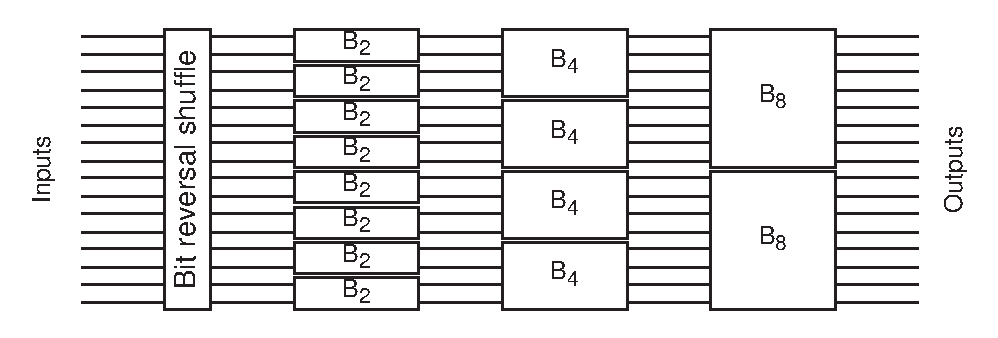
\includegraphics[width=11cm]{fftcomp}
\end{center}
\caption{FFT computation\label{Poly:FFTComp:Fig}}
\end{figure}

\smallskip
Although the algorithm described by \eqnref{FFT:Factor:Eq} appears to
be recursive, it turns out to be simpler if the column permutations
for all of the factors are performed at once.  The result is a single
reordering of the columns based on a very curious pattern.  Consider
what happens when
\eqnref{FFT:Factor:Eq} is applied twice to an $8\times8$ matrix.
Dealing only with the columns, we have
\[
A\Pi_8 = (A_0 \mid A_2 \mid A_4 \mid A_6 \mid A_1 \mid A_3 \mid A_5 \mid A_7).
\]
To apply \eqnref{FFT:Factor:Eq} to the copies of $\mathbf{F}_4$, we must
apply $\Pi_4$ to the first four columns and, separately, to the second
four columns, \ie,
\[
\begin{aligned}
(A_0 \mid A_2 \mid A_4 \mid A_6) \Pi_4 & = (A_0 \mid A_4 \mid A_2 \mid A_6),\\
(A_1 \mid A_3 \mid A_5 \mid A_7) \Pi_4 & = (A_1 \mid A_5 \mid A_3 \mid A_7),
\end{aligned}
\]
so
\[
A\Pi_8\Pi'_4 = 
  (A_0 \mid A_4 \mid A_2 \mid A_6 \mid A_1 \mid A_5 \mid A_3 \mid A_7).
\]
What has occurred is that we have sorted the columns, by the {\em bit
reversal} of their indexes.  This suggests a computational structure
as shown in \figref{Poly:FFTComp:Fig}.

\paragraph{Computational Framework}

Assume we have a vector of values $f^{(0)}_0, \ldots, f^{(0)}_{n-1}$
for which we want to compute the Fourier transform.  (We will use the
superscripts to indicate to which stage of the computation the value
corresponds.)  The first step is to reorder the $f_i$ by the bit
reversal of their indices, \ie, $f^{(1)}_i = f^{(0)}_{\mbox{rev}(i)}$,
where $\mbox{rev}(i)$ is the bit reversal of $i$.

The $f^{(1)}_i$ are now combined using a sequence of ``butterflies'' of
different sizes.  Each box in \figref{Poly:FFTComp:Fig} corresponds to
multiplication by the matrix
\[
B_r = \left(\begin{array}{cc} I_r & \Omega_r \\I_r & - \Omega_r
\end{array}\right),
\]
which we call a \keyi{butterfly}.  These matrices have precisely
two non-zero elements on each row.  Thus, when multiplying by $B_r$ we
have
\[
f^{(k+1)}_i \leftarrow f^{(k)}_i + \zeta f^{(k)}_{i+r}
\]
where $\zeta$ is an $n$-th root of unity.  It is convenient to
couple the computation of $f^{(k+1)}_i$ with that of
$f^{(k+1)}_{i+r}$:
\[
f^{(k+1)}_{i+r} \leftarrow f^{(k)}_i - \zeta f^{(k)}_{i+r}.
\]
We denote the pair of these computations by {\tt FFT2}:
\[
\mbox{\tt FFT2}[i, j, \zeta] \approx
\left\{
\left(\begin{array}{c} f^{(k+1)}_i \\ f^{(k+1)}_j \end{array}\right)
\leftarrow
\left(\begin{array}{cc} 1 & \zeta \\ 1 & -\zeta \end{array}\right)
\left(\begin{array}{c} f^{(k)}_i \\ f^{(k)}_j \end{array}\right)
\right\},
\]
where $\zeta$ is a root of unity.

The simplest computation is the 2 input butterfly, which consists of
just $\mbox{\tt FFT2}[2k, 2k+1, 1]$.  The four input butterfly
consists of two primitive computations:
\[
\mbox{\tt FFT2}[4k, 4k+2, \zeta_4^0], \mbox{\tt FFT2}[4k+1, 4k+3, \zeta_4^1],
\]
while the eight input butterfly consists of 
\[
\begin{array}{cc}
\mbox{\tt FFT2}[8k, 8k+4, \zeta_8^0],& 
  \quad \mbox{\tt FFT2}[8k+1, 8k+5, \zeta_8^1], \\
\mbox{\tt FFT2}[8k+2, 8k+6, \zeta_8^2],&
  \quad \mbox{\tt FFT2}[8k+3, 8k+7, \zeta_8^3].
\end{array}
\]

An implementation of the {\sc fft} consists of two parts: (1) a chunk of
code that shuffles the entries of $a_j$ to produce $a_j'$, and (2)
code that implements the sequence of butterflies.  In this discussion
we only discuss the second section.

The following routine replaces $f$ by its Fourier transform.  It
assumes that the length of $f$ is a power of $2$.
\begindsacode
FFT ($f$[n]) := $\{$ \\
\> FFT\=2 (i, j, $\zeta$) := $\{$ \\
\>\> $\left(\!\!\!\begin{array}{c}f\mbox{[i]}\\f\mbox{[j]}\end{array}\!\!\!\right)
  \leftarrow \left(\!\!\!\begin{array}{cc}1 & \zeta\\ 1 & -\zeta\end{array}\!\!\!\right)
  \left(\!\!\!\begin{array}{c}f\mbox{[i]}\\f\mbox{[j]}\end{array}\!\!\!\right)$;\\
\>\> $\}$; \\
\> FFT\=n (n, $k$) := $\{$ \\
\>\> unl\=ess $\mbox{n} = 2$ $\{$ \\
\>\>\> $\mbox{FFTn}(\mbox{n}/2, k)$;\\
\>\>\> $\mbox{FFTn}(\mbox{n}/2, k + \mbox{n}/2)$;\\
\>\>\> $\}$\\
\>\> loo\=p for $0 \le m < \mbox{n}/2$ do \{ \\
\>\>\> $\mbox{FFT2}(k+m, k+m+\mbox{n}/2, \zeta_{\mbox{m}})$; \\
\>\>\> $\}$ \\
\>\> $\}$ \\
\> $\mbox{FFTShuffle}(f)$; \\
\> $\mbox{FFTn}(\mbox{n}, 0)$; \\
\> $\}$
\enddsacode

\noindent
This routine uses two internal functions {\tt FFT2} and {\tt FFTn}.
{\tt FFT2} does 2 point butterfly.  The $n$ point butterfly is
implemented by the loop at the end of the {\tt FFTn}.  The first part
of {\tt FFTn} recursively computes the $n/2$ point butterflies.  

If we apply the Fourier transform and then the inverse Fourier
transform, as described by {\tt FFT}, to the same vector we will not
get the original vector, but $n$ times the original vector.  One
could deal with this problem either by adjusting the {\sc fft} routine
to remove a factor $\sqrt{n}$, or by removing a factor $n$ when
computing the inverse Fourier transform.

\medskip
One of the problems with the ``binary'' algorithm discussed in this
section is that the length of the vector transformed must be a power
of $2$.  In the years since the modern introduction of the {\sc fft}
algorithm \cite{Cooley65}, a vast number of extensions and variations
of the basic scheme discussed here have been developed.  Among these
variations are versions that permit the length of the algorithm to be
the product of small primes, \eg, $3^k$, and variations that merge the
argument shuffling we've used into the ``butterflies.''  Although all
of these methods asymptotically require $O(N \log N)$ operations, the
practical benefits they yield are very significant.

All of these {\sc fft} algorithms are valid over any field, $L$, that
contains $n$-th roots of unity.  If $L$ is either $\R$ or $\C$ then
$e^{2\pi i/n}$ can be used.  In this case, there are many good
libraries of {\sc fft} routines, including vectorized routines for
supercomputers \cite{Swarztrauber84a,Bailey87,Bailey88}.  In the case
of $L = \R$ there are variants that encode two real numbers as a
single complex number thus decreasing the number stages in the {\sc fft} by
$1$.  It is also possible to combine two real valued vectors into a
single complex complex valued vector, also decreasing the number of
arithmetic operations by a factor 2. 

When $L$ is the rational integers, $\Z$, we can continue to use
$e^{2\pi i/n}$ as a primitive $n$-th root of unity\index{primitive root!of unity} if the round-off
errors introduced are carefully analyzed.  This is not the case when
$L$ is a finite field.  Assume that $L = \F_q$, so every element of
$L$ is a zero of $X^{q-1} - 1$, \ie, every element of $L$ is a root of
unity.  If $n$ divides $q-1$ then, by the discussion in
\sectref{FF:Multiplicative:Sec}, $L$ has $\phi(n)$ elements of order
$n$.  Each of these is a primitive $n$-th root of unity.   

If one needs an $n$-th root of unity that does not lie in $\F_q$,
then it can always be obtained by adjoining zeroes of irreducible
factors of $X^n-1$ to $\F_q$.  This however, can be quite expensive.
For instance, to interpolate a polynomial of degree $63$ over $\F_5$,
we need a $64$-th root of unity.  The smallest field of
characteristic $5$ with $64$-th roots of unity is $\F_{5^{16}}$.
Arithmetic in this field is at least $16 \log 16 = 64$ times more
expensive than arithmetic in $\F_5$.  So, the {\sc fft} approach here
is not likely to be of benefit.

\paragraph{FFT Based Interpolation}

The fast Fourier transform routine, {\tt FFT}, allows us to
interpolate the right type of black boxes exceedingly quickly.  Assume
that ${\cal B}_P$ represents a polynomial of degree $d$ over a field
$L$.  Let $n$ be $\lceil \log_2 d \rceil$ and assume that $\zeta \in
L$ is a primitive root of unity\index{primitive root!of unity} of
order $N = 2^n$.  Construct the set of values
\[
{\cal B}_P(1), {\cal B}_P(\zeta), {\cal B}_P(\zeta^2), {\cal
B}_P(\zeta^3), \ldots, {\cal B}_P(\zeta^{2^n-1}).
\]
The Fourier transform of this sequence will be the coefficients of
$P$.  The last $2^n - d$ of them should be zero.

The time required of this approach is $N = 2^{\lceil \log_2 d
\rceil}$ evaluations and $O(N \log N) = O(d \log d)$ operations for 
the {\sc fft}.

\medskip
It is informative to analyze the case of $L = \Z$ in a bit more
detail.  Assume that we are also given $B \ge |P|$, a bound on the
absolute value of the coefficients of $P$, in addition to $n$, a power
of two that bounds the degree of $P$.  Instead of performing the
interpolation over $\R$, we can instead choose a set of fields
$\F_{q_1}, \ldots, \F_{q_k}$, of characteristic $p_1, \ldots, p_k$
such that $n \mid (q_i -1)$ and such that $p_1 \cdots p_k \ge 2B + 1$.
Using $k \cdot n$ evaluations of ${\cal B}_P$ we can compute the image
of $P$ modulo the $p_i$.  The \key{Chinese remainder theorem} can now be
used to reconstruct $P$ over the integers.  The time required by such
an approach is
\[
O(k n \log n + n M_{\rm int}(\log B)^2)
\]
where $M_{\rm int}(\log B)$ is the time to multiply to integers of
$\log B$ bits.  Again this is asymptotically faster than the simpler,
Lagrangian and Newtonian interpolation algorithms discussed earlier,
but practically it is not of use except for univariate polynomials of
large degree.

\paragraph{Fast Polynomial Multiplication}

Let $F(X)$ and $G(X)$ be two polynomials over degree $m$ over a field
$L$,
\[
\begin{aligned}
  F(X) &= f_{m-1} X^{m-1} + f_{m-2} X^{m-2} + \cdots + f_0,\\
  G(X) &= g_{m-1} X^{m-1} + g_{m-2} X^{m-2} + \cdots + g_0.
\end{aligned}
\]
We want to compute $H(X) = F(X) G(X)$, were $\deg H = n = 2m$.  Using
classical multiplication we can do this using $O(n^2)$
multiplications.  We would like to do better using interpolation. 

We can easily construct a black box for $H$, ${\cal B}_H(x) = F(X)
G(x)$, when $x \in L$.  By choosing $n$ values of $x$ and using the
univariate interpolation techniques discussed earlier, we can
reconstruct $H$.  The cost however is still $O(n^2)$ multiplications.
Each evaluation of ${\cal B}_H$ requires $O(n)$ multiplications, so it
takes $O(n^2)$ multiplications to compute all of the values.  The
Newtonian and Lagrangian interpolation schemes themselves require
$O(n^2)$ operations.

However, by using the fast Fourier transform we can do better.  The
interpolation cost immediately drops from $O(n^2)$ to $O(n \log n)$.
In addition, we can compute all of the values of $F(X)$ and $G(X)$
using a single fast Fourier transform for each.  Thus we can bring the
total asymptotic cost of polynomial multiplication down to $O(n \log
n)$.  This technique for multiplying polynomials is the most efficient
known thus far.  However, all of the practical problems alluded to in
the previous section apply here also.  These problems are exacerbated
when dealing with multivariate polynomials, which frequently occur.

On the other hand, for moderate to large degree univariate polynomials
with coefficients in $\R$, $\C$, or, perhaps, small elements of $\Z$,
the {\sc fft} method can be quite effective.  When $L = \R$ this is
especially true if one uses an {\sc fft} routine that determines the
transform of two real functions at once using a single complex
transform.

\index{fast Fourier transform|)}


\section{Abstract Interpolation} 
\label{Interp:Abstract:Sec}

In this section we introduce a bit more abstraction into our
discussion of interpolation.  This will allow us to deal with a
variety of different types of interpolation problems in a uniform
framework.

Let $R$ be a commutative ring with unit and let $\mathfrak{m}$ be an
ideal of $R$.  Recall that $R/\mathfrak{m}$ is set of residue classes of
$R$ modulo $\mathfrak{m}$.  Two elements of $R$ $x$ and $y$ are in the
same equivalence class in $R/\mathfrak{m}$ if $x - y$ is an element of
the ideal $\mathfrak{m}$.  There is a natural map that sends elements of
$R$ to the equivalence classes in which they lie in $R/\mathfrak{m}$.
This map induces a ring structure on $R/\mathfrak{m}$.  If $\mathfrak{m}$ is
a \key{prime ideal} then $R/\mathfrak{m}$ is an \key{integral domain}.
If $\mathfrak{m}$ is a \key{maximal ideal} then $R/\mathfrak{m}$ is a field.

For many rings $R$ and ideals $\mathfrak{m}$ there is a canonical
representative for each class in $R/\mathfrak{m}$.  In such cases, we use
the canonical representative and the equivalence class
interchangeably.

Two common examples are $R = \Z$ and $R = L[X]$, where $L$ is a field.
The ideals of $\Z$ are principal, \ie, all ideals are generated by a
single element, $\mathfrak{m} = (m)$.  The canonical representatives of
the equivalence classes of the quotient ring $\Z/(m)$ are the integers
$\{0, 1, \ldots, m-1\}$ (using the \key{one sided presentation} of
\chapref{Finite:Fields:Chap}).  The prime ideals of $\Z$ are also
maximal.  If $m$ is prime them $\Z/(m)$ is a field.  If on the
other hand, $m$ is divisible by $p > 1$, then $p$ will be a zero
divisor and $Z/(m)$ cannot be an integral domain.

The ideals of $L[X]$ are also principal, but are generated by the
polynomials in $L[X]$.  Let $\mathfrak{m} = (m(X))$ be an ideal in
$L[X]$.  Since $L$ is a field, we can assume that $m(X)$ is monic.  As
with $\Z$, the canonical representatives in $L[X]/\mathfrak{m}$ are the
reduced residues modulo $m(X)$.  The case when $m(X)$ is linear occurs
frequently.  Let $a(X) \in L[X]$ be a polynomial, and assume $m(X) = X
- k$, where $k$ is an element of $L$.  The remainder of $a(X)$ when
divided by $X - k$ is $a(k)$.

For $a$ an element of a ring $R$, and $\mathfrak{m}$ an ideal of $R$, we
use the notation
\[
a(\mathfrak{m}) = a \mod\mathfrak{m}.
\]
Thus, if $\mathfrak{m} = (X - k)$ then $a(k) = a(\mathfrak{m}) = a((X -
k))$.  Note the extra set of parenthesis in the last form, which will
not be often used.  

\medskip
With this notation we can discuss interpolation in a manner that
strengthens the parallels between the Chinese remainder algorithm for
integers of \sectref{Integer:Chinese:Remainder:Sec} and that for
polynomials in \sectref{Interp:CRA:Sec}.  The following is the
standard version of the \key{Chinese remainder theorem}

\begin{proposition}[Chinese Remainder Theorem]
Let $\mathfrak{p}_1, \ldots, \mathfrak{p}_n$ be ideals in a ring $R$, such
that every pair is co-prime, \ie, $\mathfrak{p}_i + \mathfrak{p}_j = (1)$ if
$i\not=j$.  There is a one to one correspondence between $n$-tuples in
$R/\mathfrak{p}_1 \times \cdots \times R/\mathfrak{p}_n$ and $R/\mathfrak{p}_1
\cdots \mathfrak{p}_n$.
\end{proposition}

Let $\mathfrak{p}_1, \ldots, \mathfrak{p}_t$ be ideals in $R$ and $F$
be an element of $R$.  The interpolation problem is: Given
$F(\mathfrak{p}_1), \ldots, F(\mathfrak{p}_t)$ compute an element of
$R/\mathfrak{p}_1 \cdots \mathfrak{p}_t$ whose image in
$R/\mathfrak{p}_i$ is $F(\mathfrak{p}_i)$.  In the context of black
boxes, we have a black box ${\cal B}_F$ that accepts an ideal
$\mathfrak{q}$ and returns ${\cal B}_F(\mathfrak{q}) = F(\mathfrak{q})$.
Again our goal is reconstruct $F$.

Consider the simple case where there are only two ideals $\mathfrak{p}$
and $\mathfrak{q}$.  We are given $F(\mathfrak{p})$ and $F(\mathfrak{q})$ and
we want to compute $F(\mathfrak{pq})$.  Recall that when $R = \Z$ it was
necessary to require that the two moduli be relatively prime.  With
ideals, the same constraint is that $\mathfrak{p} + \mathfrak{q} = 1$.  That
is, there exist $a \in \mathfrak{p}$ and $b \in \mathfrak{q}$ such that
$a+b=1$.  Thus
\[
F(\mathfrak{pq}) = a F(\mathfrak{p}) + b F (\mathfrak{q}).
\]

In more generality, let $\mathfrak{p}_1, \ldots, \mathfrak{p}_t$ be pairwise
co-prime ideals in $R$ and define
\[
\mathfrak{P}_i = \mathfrak{p}_1 \cdots \mathfrak{p}_{i-1} \mathfrak{p}_{i+1}
\cdots \mathfrak{p}_t.
\]
The $\mathfrak{P}_i$ are defined so that 
\[
\mathfrak{P}_1 + \mathfrak{P}_2 + \cdots + \mathfrak{P}_t = (1)
\]
any smaller subset is divisible by some $\mathfrak{p}_j$.  Letting $p_i$
be elements of $\mathfrak{P}_i$ whose sum is $1$ gives,
\begin{equation}\label{CRA:Lagrange:Eq}
F(\mathfrak{p}_1 \cdots \mathfrak{p}_t) = 
 p_1 F(\mathfrak{p}_1) + p_2 F(\mathfrak{p}_2) + \cdots +
  p_t F(\mathfrak{p}_t).
\end{equation}

When $R = k[Z]$ this is precisely the \key{Lagrange interpolation
formula} discussed earlier.  Let $\mathfrak{p}_i = (Z - z_i)$, so
\[
\mathfrak{P}_i = \left((Z - z_0) \cdots (Z-z_{i-1})(Z-z_{i+1}) \cdots
(Z-z_t)\right)
\]
and
\[
p_i = \frac{(Z-z_0)\cdots(Z - z_{i-1})(Z - z_{i+1}) \cdots (Z-z_t)}{(z_i-z_0)\cdots(z_i - z_{i-1})(z_i - z_{i+1}) \cdots (z_i-z_t)}.
\]
The sum of the $p_i$ is a polynomial of degree $t$.  Its value at $Z =
z_0, z_1, \ldots, z_t$ is $1$ so it must be identically equal to $1$.

A Lagrangian interpolation formula can be developed for $R = \Z$ by
using \eqnref{CRA:Lagrange:Eq}.  Consider the simple case of two
ideals, $\mathfrak{p} = (p)$ and $\mathfrak{q} = (q)$.  Again, we are
looking for $a \in \mathfrak{p}$ and $b \in \mathfrak{q}$ such that $a+b =
1$ modulo $\mathfrak{pq}$.  Since  $a = xp$ and $b = yq$, we want to find
$x$ and $y$ such that 
\begin{equation} \label{Abs:Dio:Eq}
xp + yq = 1,
\end{equation}
where $x$ and $y$ are integers.  As we know this diophantine equation
has solutions if and only if $p$ and $q$ are relatively prime.  Let
$\bar{x}$ and $\bar{y}$ be solutions of \eqnref{Abs:Dio:Eq}.

If we have
\[
\begin{aligned}
F &= k_1 \pmod{p} \\
F &= k_2 \pmod{q}
\end{aligned}
\]
Then a Lagrangian interpolation formula for $F$ is
\[
F = \bar{x} \cdot  k_2 \cdot p + \bar{y} \cdot k_1 \cdot q \pmod{pq}.
\]

\section*{Notes}

\small

\notesectref{Vandermonde:Sec} \propref{Gen:Vandermonde:Prop} appears
in {\Polya} and {\Szego} \cite{Polya:Szego}, Chapter 5, problem 48.
Additional partial results on generalized Vandermonde matrices are
contained in the work of {\MitchellO} \cite{Mitchell:Vandermonde}, and
{\EvansR} and {\Isaacs} \cite{Evans:Generalized:Vandermonde}.

\notesectref{Poly:FFT:Sec}
The fast Fourier transform algorithm was first discussed in modern
terms by {\Cooley} and {\Tukey} \cite{Cooley65}, although the basic
ideas have been known by a variety of authors starting with {\Gauss}.
See \cite{Heideman84} for a historical survey.  More detailed
discussions of fast Fourier transform algorithms and their
applications are contained in 
\cite{Tolimieri89,Brigham88,VanLoan92,Pollard71}.

{\CantorD} and {\Kaltofen} \cite{Cantor91} have generalized the {\sc fft}
polynomial multiplication technique to polynomials over arbitrary
algebras.  For univariate polynomials of degree $n$, their technique
requires $O(n \log n)$ multiplies and $O(n \log n \log \log n)$
additions.

Bonneau has studied the use of {\sc fft} to speed polynomial
multiplication
\cite{Bonneau:Thesis}.

\normalsize
